%%
% This is an Overleaf template for presentations
% using the TUM Corporate Desing https://www.tum.de/cd
%
% For further details on how to use the template, take a look at our
% GitLab repository and browse through our test documents
% https://gitlab.lrz.de/latex4ei/tum-templates.
%
% The tumbeamer class is based on the beamer class.
% If you need further customization please consult the beamer class guide
% https://ctan.org/pkg/beamer.
% Additional class options are passed down to the base class.
%
% If you encounter any bugs or undesired behaviour, please raise an issue
% in our GitLab repository
% https://gitlab.lrz.de/latex4ei/tum-templates/issues
% and provide a description and minimal working example of your problem.
%%

\documentclass[
  german,            % define the document language (english, german)
  aspectratio=169,    % define the aspect ratio (169, 43)
  % handout=2on1,       % create handout with multiple slides (2on1, 4on1)
  % partpage=false,     % insert page at beginning of parts (true, false)
  % sectionpage=true,   % insert page at beginning of sections (true, false)
]{tumbeamer}


% load additional packages
\usepackage{booktabs}
\usepackage{graphicx}
\usepackage{tikz}
\usepackage{url}
\usepackage{pgfplots}
\usepackage{hyperref}
\usepackage{pmboxdraw}
\usepackage{float}
\usepackage{babel}[ngerman]
\usepackage{csquotes}[autostyle]
\usepackage[useregional]{datetime2}
\usepackage{listings}
% Copied from Markus Gschoßmann
%
% RISC-V Assembler syntax and style for latex lstlisting package
% 
% These are risc-v commands as per our university (University Augsburg, Germany) guidelines.
%
% Author: Anton Lydike
%
% This code is in the public domain and free of licensing

% language definition

\usepackage{listings}

\lstdefinelanguage[RISC-V]{Assembler}
{
  alsoletter={.}, % allow dots in keywords
  alsodigit={0x}, % hex numbers are numbers too!
  morekeywords=[1]{ % instructions
    lb, lh, lw, lbu, lhu,
    sb, sh, sw,
    sll, slli, srl, srli, sra, srai,
    add, addi, sub, lui, auipc,
    xor, xori, or, ori, and, andi,
    slt, slti, sltu, sltiu,
    beq, bne, blt, bge, bltu, bgeu,
    j, jr, jal, jalr, ret,
    scall, break, nop,
    mul, mulh, mulhu, mulhsu,
    li
  },
  morekeywords=[2]{ % sections of our code and other directives
    .align, .ascii, .asciiz, .byte, .data, .double, .extern,
    .float, .globl, .half, .kdata, .ktext, .set, .space, .text, .word
  },
  morekeywords=[3]{ % registers
    zero, ra, sp, gp, tp, s0, fp,
    t0, t1, t2, t3, t4, t5, t6,
    s1, s2, s3, s4, s5, s6, s7, s8, s9, s10, s11,
    a0, a1, a2, a3, a4, a5, a6, a7,
    ft0, ft1, ft2, ft3, ft4, ft5, ft6, ft7,
    fs0, fs1, fs2, fs3, fs4, fs5, fs6, fs7, fs8, fs9, fs10, fs11,
    fa0, fa1, fa2, fa3, fa4, fa5, fa6, fa7
  },
  morecomment=[l]{;},   % mark ; as line comment start
  morecomment=[l]{\#},  % as well as # (even though it is unconventional)
  morestring=[b]",      % mark " as string start/end
  morestring=[b]'       % also mark ' as string start/end
}

% define some basic colors
\definecolor{mauve}{rgb}{0.58,0,0.82}

\lstset{
  % listings sonderzeichen (for german weirdness)
  literate={ö}{{\"o}}1
           {ä}{{\"a}}1
           {ü}{{\"u}}1,
  basicstyle=\tiny\ttfamily,                    % very small code
  breaklines=true,                              % break long lines
  commentstyle=\itshape\color{green!50!black},  % comments are green
  keywordstyle=[1]\color{blue!80!black},        % instructions are blue
  keywordstyle=[2]\color{orange!80!black},      % sections/other directives are orange
  keywordstyle=[3]\color{black!50!black},       % registers are black
  stringstyle=\color{mauve},                    % strings are from the telekom
  identifierstyle=\color{teal},                 % user declared addresses are teal
  frame=l,                                      % black line on the left side of code
  language=[RISC-V]Assembler,                   % all code is RISC-V
  tabsize=4,                                    % indent tabs with 4 spaces
  showstringspaces=false                        % do not replace spaces with weird underlines
}


\lstset {
    frame=single,
    tabsize=4,
    breaklines=true,
    xleftmargin=5pt,
    xrightmargin=5pt,
    basicstyle=\ttfamily\footnotesize,
    %language=[RISC-V]Assembler,
}

\hypersetup { 
  colorlinks=true,
  urlcolor=blue,
  filecolor=black,
  linkcolor=black
}

% tikz  
\usetikzlibrary{fit}

% image path
\graphicspath{ {../resources/} }

% presentation metadata
\title{Übung 03: RISC-V Deep Dive}
\subtitle{Einführung in die Rechnerarchitektur}
\author{\theAuthorName}

\institute{\theGroupName\\\theSchoolName\\\theUniversityName}
\date{04. -- \DTMdisplaydate{2024}{11}{10}{-1}}

\footline{\insertauthor~|~\insertshorttitle~|~\insertshortdate}


% macro to configure the style of the presentation
\TUMbeamersetup{
  title page = TUM tower,         % style of the title page
  part page = TUM toc,            % style of part pages
  section page = TUM toc,         % style of section pages
  content page = TUM more space,  % style of normal content pages
  tower scale = 1.0,              % scaling factor of TUM tower (if used)
  headline = TUM threeliner,      % which variation of headline to use
  footline = TUM default,         % which variation of footline to use
  % configure on which pages headlines and footlines should be printed
  headline on = {title page},
  footline on = {every page, title page=false},
}


% available frame styles for title page, part page, and section page:
% TUM default, TUM tower, TUM centered,
% TUM blue default, TUM blue tower, TUM blue centered,
% TUM shaded default, TUM shaded tower, TUM shaded centered,
% TUM flags
%
% additional frame styles for part page and section page:
% TUM toc
%
% available frame styles for content pages:
% TUM default, TUM more space
%
% available headline options:
% TUM empty, TUM oneliner, TUM twoliner, TUM threeliner, TUM logothreeliner
%
% available footline options:
% TUM empty, TUM default, TUM infoline


\begin{document}

\maketitle

\begin{frame}[c]{Mitschriften \& Infos}{}
  \begin{minipage}[t]{\textwidth}
    \begin{columns}[c]
      \begin{column}{0.8\textwidth}
        Montags: \href{\zulipMo}{\zulipMo}
      \end{column}
      \begin{column}{0.2\textwidth}
        \includegraphics[width=0.8\linewidth]{\zulipMoQrFilename}
      \end{column}
    \end{columns}
  \end{minipage}
  \rule{\textwidth}{0.4pt}
  \begin{minipage}[t]{\textwidth}
    \begin{columns}[c]
      \begin{column}{0.8\textwidth}
        Donnerstags: \href{\zulipDo}{\zulipDo}
      \end{column}
      \begin{column}{0.2\textwidth}
        \includegraphics[width=0.8\linewidth]{\zulipDoQrFilename}
      \end{column}
    \end{columns}
  \end{minipage}
  \ifdefined\myWebsite
  \rule{\textwidth}{0.4pt}
  \centering
  Website: \href{\myWebsite}{\myWebsite}
  \fi
\end{frame}

\begin{frame}[c]{}{}
  \begin{center}
    \LARGE  Keine Garantie für die Richtigkeit der Tutorfolien.

    \Large Bei Unklarheiten/Unstimmigkeiten haben VL/ZÜ-Folien recht!
  \end{center}
\end{frame}

\begin{frame}[c]{Inhaltsübersicht}{}
  \begin{columns}[c]
    \begin{column}{1\textwidth}
      \begin{itemize}
        \item Quiz
        \item Musterlösung der Hausaufgabe
        \item Kurze Wiederholung
        \item Tutorblatt
        \begin{itemize}
          \item Arrays und deren Adressierung
          \item Zeichenketten/Strings
          \item Taschenrechner-Tester (Präsenzaufgabe 01)
        \end{itemize}
      \end{itemize}
    \end{column}
  \end{columns}
\end{frame}

\begin{frame}[c]{}{}
  \begin{center}
    \LARGE Hausaufgabe: H02 - Festkommarechnung
  \end{center}
\end{frame}

\begin{frame}[fragile]{Hausaufgabe 02: mul\_pi\_16\_16}
  \framesubtitle{Code}
  \begin{lstlisting}
  # pi in 16.16 (pi*65536)
  li a1, 0x3243F
  # high 32 bit of result
  mulhu t1, a0, a1
  # low 32 bit of result
  mul t0, a0, a1
  # get middle 32 bit by shifts and or
  srli t0, t0, 16
  slli t1, t1, 16
  or a0, t0, t1
  # return
  jalr zero, 0(ra)
  \end{lstlisting}
\end{frame}

\begin{frame}[fragile]{Hausaufgabe 02: mul\_n\_fixed\_point}
  \framesubtitle{Code}
  \begin{lstlisting}
  #store lower 32bits into a3
  mul a3, a0, a1
  #store higher 32bits into a4
  mulhu a4, a0, a1
  #store temporary the number 32 for next step
  addi a5, zero, 0x20
  #get number of bits before ,
  sub a6, a5, a2
  #handle special case, if numbers are in format 32.0
  beq a2, zero, zero_bit_decimal
  #handle special case, if numbers are in format 0.32
  beq a6, zero, thirtytwo_bit_decimal
  #shift lower 32-bits to the right by number of decimal places
  srl a3, a3, a2
  \end{lstlisting}
\end{frame}

\begin{frame}[fragile]{Hausaufgabe 02: mul\_n\_fixed\_point}
  \framesubtitle{Code}
  \begin{lstlisting}
    #shift higher 32-bits to the left by 32-(a2)
    sll a4, a4, a6
    #concat shifted lower and higher bits with or
    or a0, a3, a4
    # return
    jalr zero, 0(ra)
  #if format is 32.0, the whole result is in a3 (result of mul)
  zero_bit_decimal:
    #load result from a3 to a0
    add a0, zero, a3
    jalr zero, 0(ra)
  #if format is 0.32, the whole result is in a4 (result of mulhu)
  thirtytwo_bit_decimal:
    add a0, zero, a4
    jalr zero, 0(ra)
  \end{lstlisting}
\end{frame}

\begin{frame}[c]{}{}
  \begin{center}
    \LARGE  Wiederholung
  \end{center}
\end{frame}

\begin{frame}[c]{Register \& Calling Convention}{}
  \begin{columns}[c]
    \begin{column}{0.5\textwidth}
      \begin{itemize}
        \item Argumente: a0 bis a5
        \item Rückgabewert: In a0 - a1 erwartet
        \item Temporäre Register: t0 - t6 können einfach überschrieben werden
        \item Saved Registers: s0 - s11 können genutzt werden, müssen vor return aber wiederhergestellt werden
      \end{itemize}
    \end{column}
    \begin{column}{0.5\textwidth}
      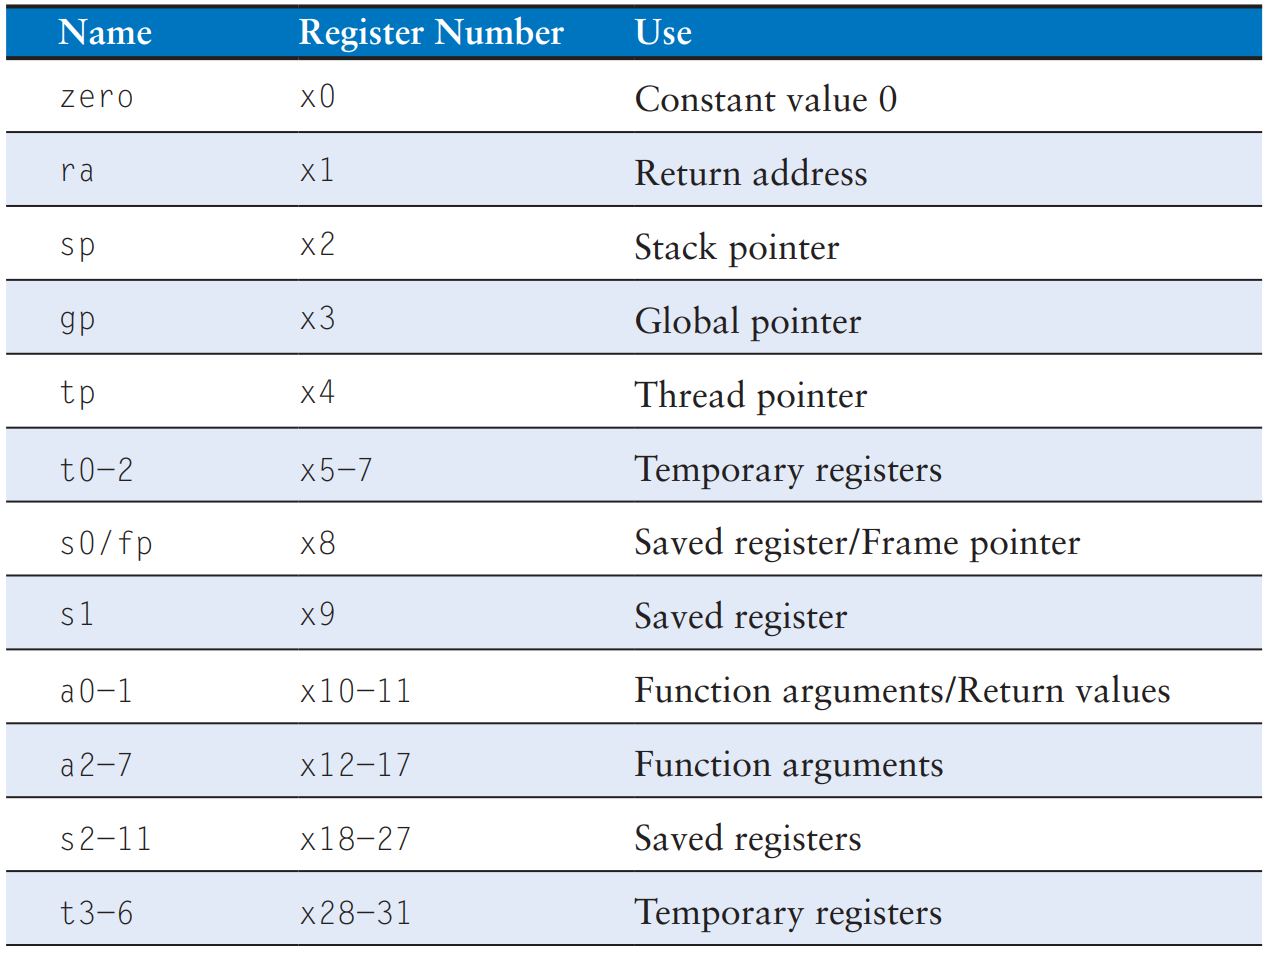
\includegraphics[width=\linewidth]{riscv_registers.png}
    \end{column}
  \end{columns}
\end{frame}

\begin{frame}[c]{Wichtige Instruktionen}{}
  \centering
  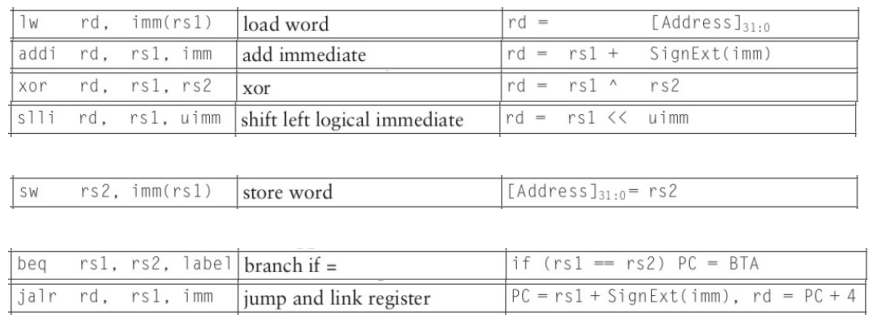
\includegraphics[width=\linewidth]{w03_integerinstructions.png}
\end{frame}

\begin{frame}[c]{If-else in RISC-V}{}
  \centering
  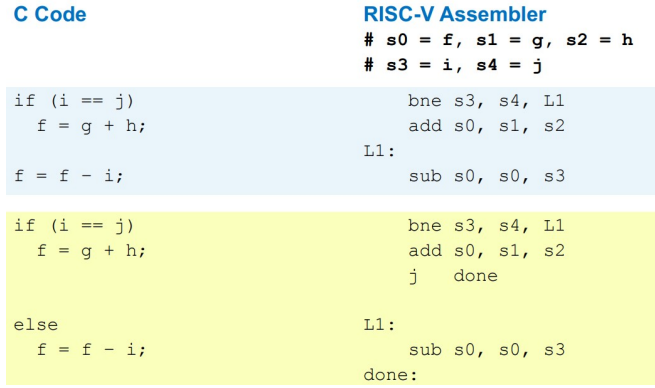
\includegraphics[width=0.75\linewidth]{w03_ifelseassembly.png}
\end{frame}

\begin{frame}[c]{While in RISC-V}{}
  \centering
  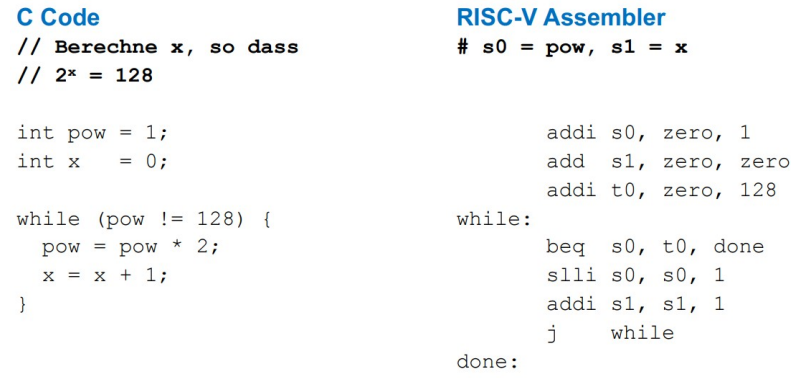
\includegraphics[width=0.8\linewidth]{w03_whileassembly.png}
\end{frame}

\begin{frame}[c]{Speicherorganisation}{}
  \begin{columns}[c]
    \begin{column}{0.5\textwidth}
      \begin{itemize}
        \item \#todo
      \end{itemize}
    \end{column}
    \begin{column}{0.5\textwidth}
      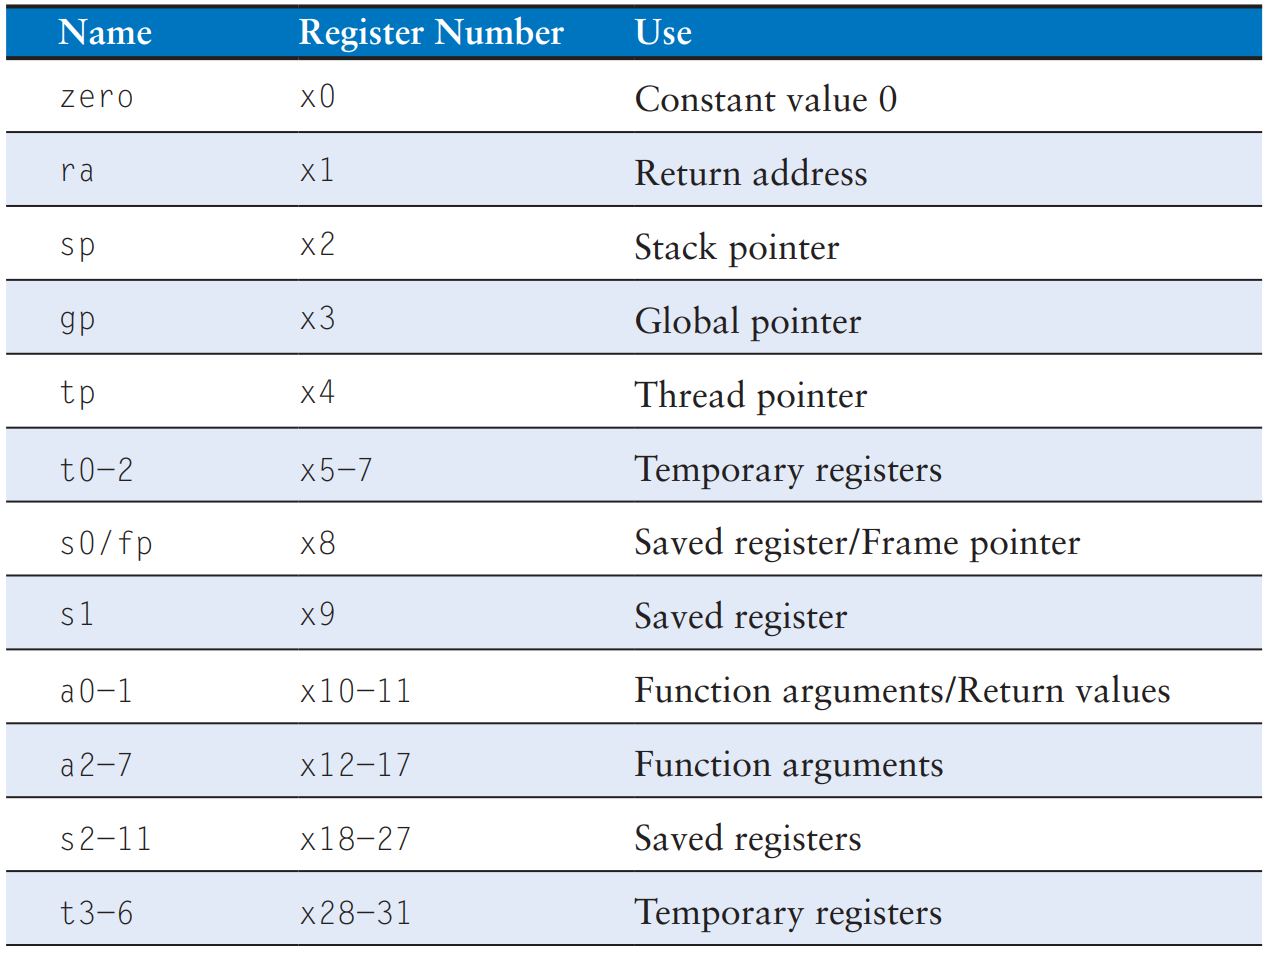
\includegraphics[width=\linewidth]{riscv_registers.png}
    \end{column}
  \end{columns}
\end{frame}

\begin{frame}[c]{Strings sind Arrays}{}
  \begin{columns}[c]
    \begin{column}{0.5\textwidth}
      \begin{itemize}
        \item Strings sind nur Arrays aus Buchstaben
        \item Im Computer sind die Buchstaben durch Zahlen repräsentiert
        \item Zeichen sind ASCII enkodiert (0-127)
        \item 2 verschiedene Arten von Strings
        \begin{itemize}
          \item C-Strings: Aneinanderreihung von Zeichen dann NULL-Byte
          \item Pascal-Strings: Erst 1 Byte für die Länge des Strings, dann Zeichen
        \end{itemize}
      \end{itemize}
    \end{column}
    \begin{column}{0.5\textwidth}
      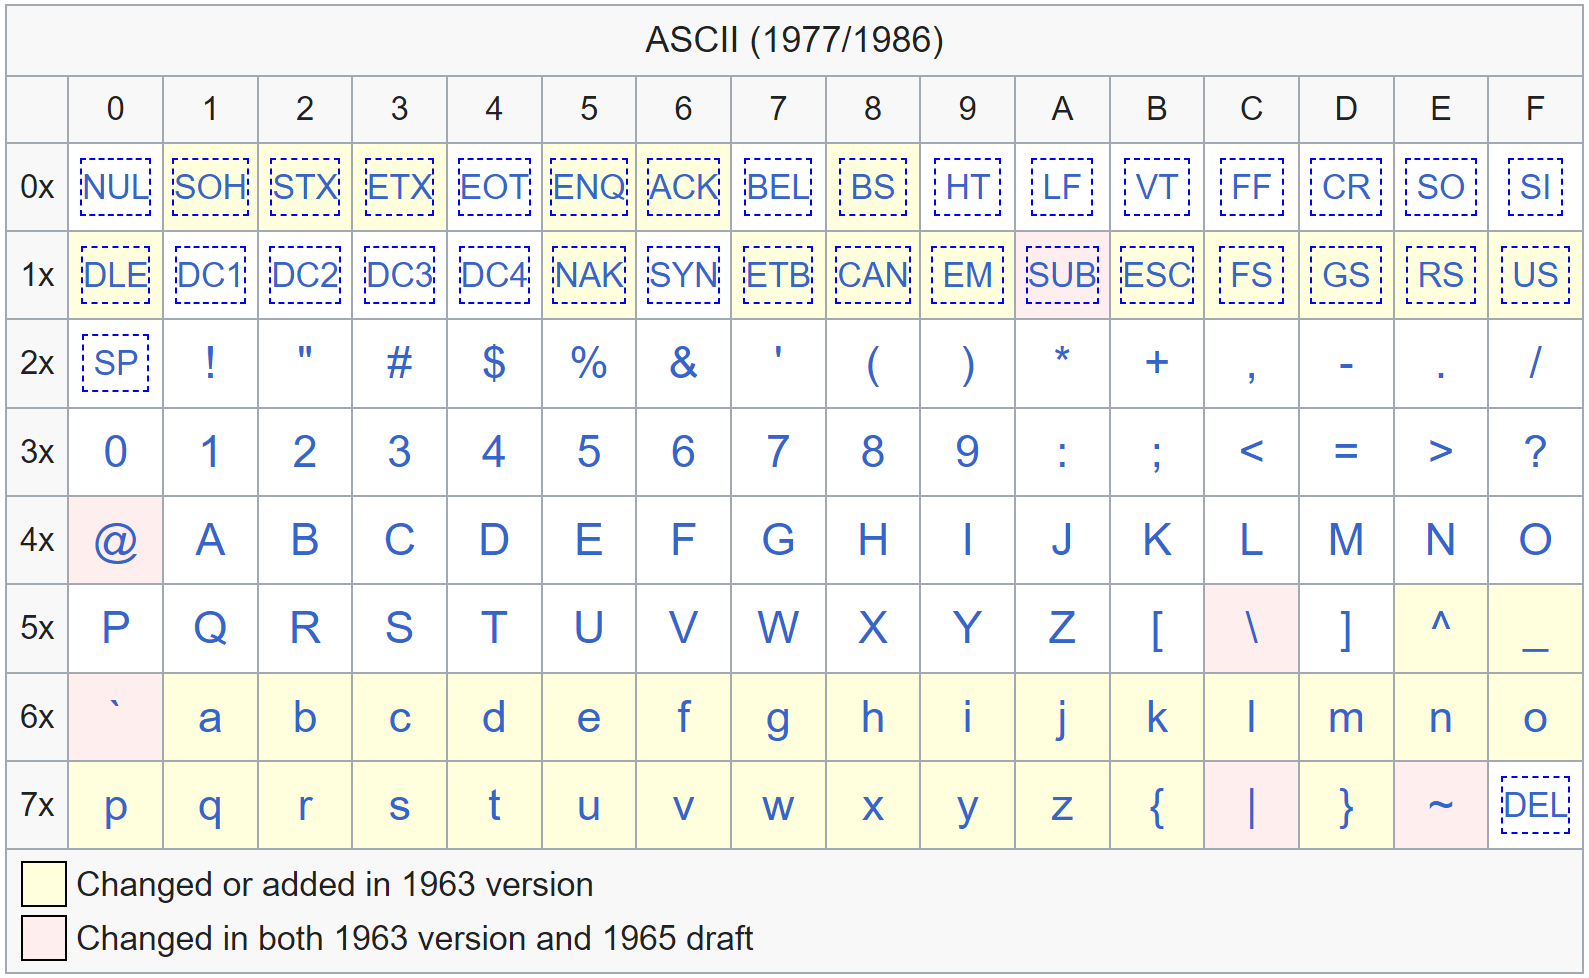
\includegraphics[width=\linewidth]{ascii.png}
    \end{column}
  \end{columns}
\end{frame}

\begin{frame}[c]{Structs}{}
  \begin{columns}[c]
    \begin{column}{0.5\textwidth}
      \begin{itemize}
        \item \#todo
      \end{itemize}
    \end{column}
    \begin{column}{0.5\textwidth}
      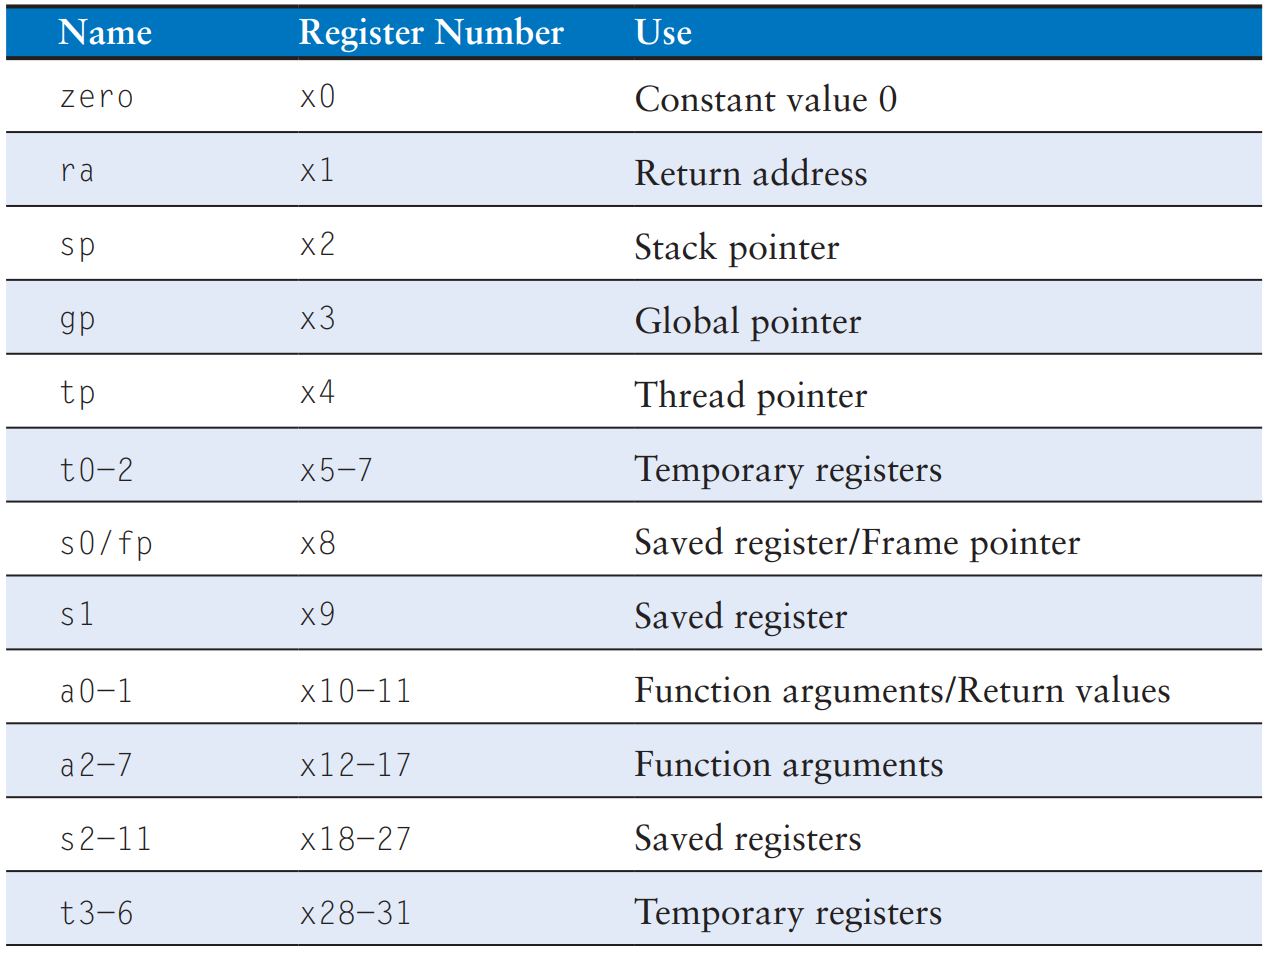
\includegraphics[width=\linewidth]{riscv_registers.png}
    \end{column}
  \end{columns}
\end{frame}

\begin{frame}[c]{Sections}{}
  \begin{columns}[c]
    \begin{column}{0.5\textwidth}
      \begin{itemize}
        \item \#todo
      \end{itemize}
    \end{column}
    \begin{column}{0.5\textwidth}
      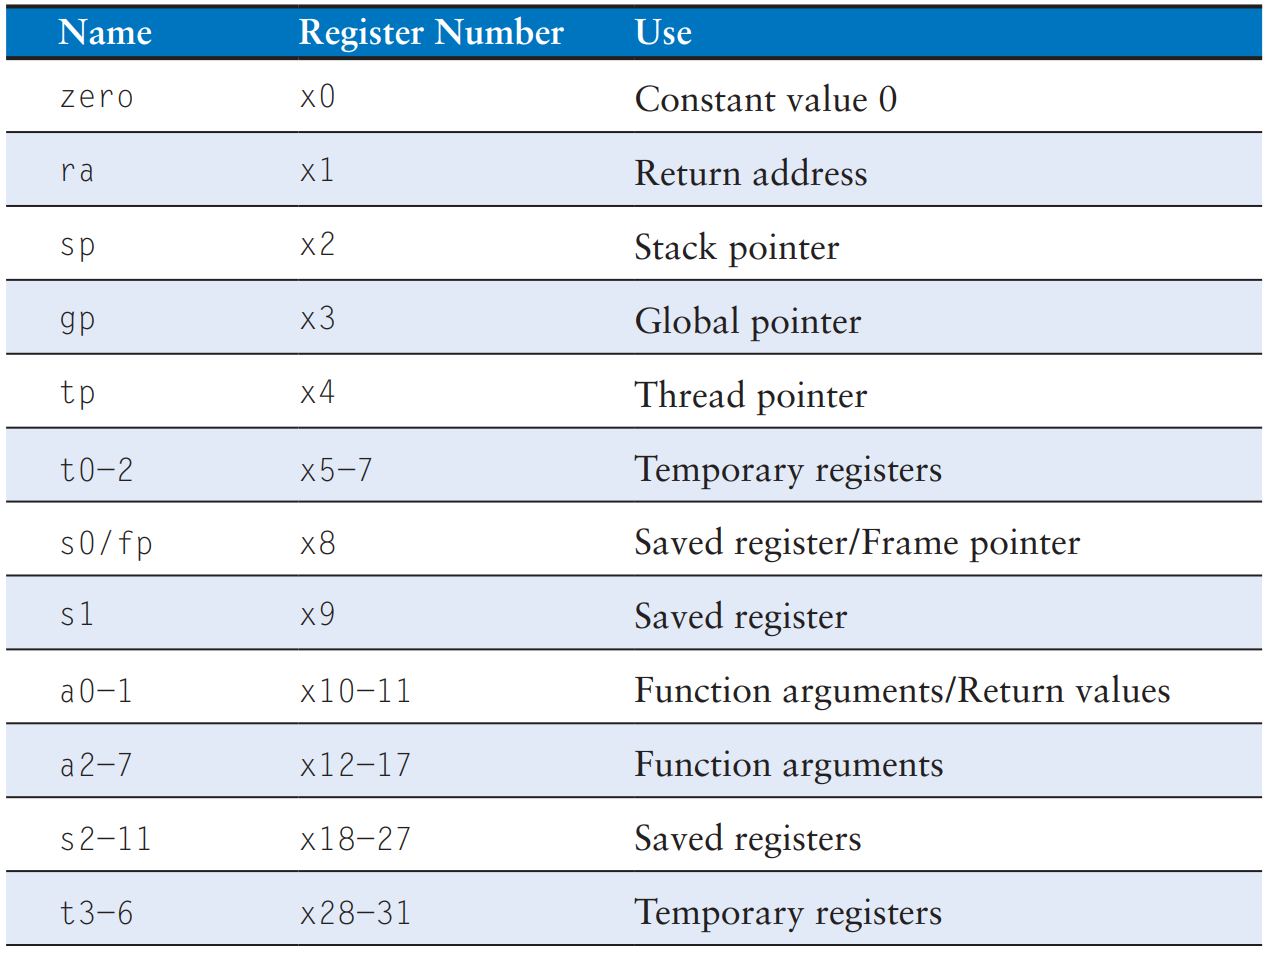
\includegraphics[width=\linewidth]{riscv_registers.png}
    \end{column}
  \end{columns}
\end{frame}

\begin{frame}[c]{}{}
  \begin{center}
    \LARGE Fragen?
  \end{center}
  \vspace{0.5cm}
  \begin{center}
    \LARGE Bis zum nächsten Mal ;) \\
  \end{center}
  \vspace{1.0cm}
  \begin{center}
    \small Folien inspiriert von Markus Gschoßmann und Clemens Schwarzmann
  \end{center}
\end{frame}

\end{document}